\section{Annotation des sections et entités judiciaires}

\subsection{Objectif}
\begin{frame}[c]{Références dans l'entête, normes dans le reste}
\begin{figure}
	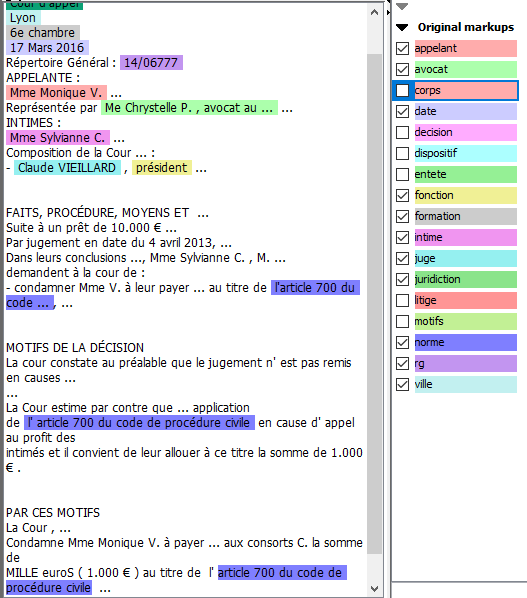
\includegraphics[height=\textheight]{decision-marquee.png}
\end{figure}
\end{frame}

\begin{frame}{Sectionner les décisions pour organiser l'extraction}
\scriptsize
\begin{columns}
	\begin{column}{.45\linewidth}
		\fbox{\begin{minipage}{\textwidth}ARRÊT N°
				
				R.G: \textcolor{red}{11/03924}
				
				\textcolor{red}{COUR D'APPEL} DE \textcolor{red}{NÎMES}
				
				\textcolor{red}{CHAMBRE CIVILE}
				
				\textcolor{red}{1ère Chambre A}
				
				ARRÊT DU \textcolor{red}{20 MARS 2012}
				
				APPELANTE:
				
				\textcolor{red}{Madame Michéle A.} ...
				
				assistée de la \textcolor{red}{SELARL VAJOU}, ...
				
				INTIMES:
				
				\textcolor{red}{Monsieur Martial B} ...
				
				assisté de la \textcolor{red}{SCP MARION GUIZARD PATRICIA SERVAIS}, ...
				
				COMPOSITION DE LA COUR LORS DU DÉLIBÉRÉ:
				
				\textcolor{red}{M. Dominique BRUZY, Président}
				
				\textcolor{red}{M. Serge BERTHET, Conseiller}
				
				...
		\end{minipage}}
		\vspace{0.1cm}
		
		{\normalsize \textbf{Entêtes}: méta-données}
	\end{column}
	\begin{column}{.55\linewidth}
		\fbox{\begin{minipage}{\textwidth}FAITS, PROCEDURE, ...
				
				Madame Michèle A. demande:
				
				...
				
				- de condamner Madame JONES-B. à lui payer la somme de \textcolor{red}{2.500 euros} au titre de l'\textcolor{red}{article 700 du Code de Procédure Civile}, 
		\end{minipage}}
		\vspace{0.1cm}
		
		{\normalsize \textbf{Corps}: demandes, arguments et normes }
		
		\vspace{0.4cm}
		
		\fbox{\begin{minipage}{\textwidth}PAR CES MOTIFS, LA COUR:
				
				...
				
				Vu l'\textcolor{red}{article 809 du Code de Procédure Civile},
				
				...
				
				\textcolor{red}{Déboute Madame A. de sa demande de provision sur dommages-intérêts.}
				
				...
				
				Vu l'\textcolor{red}{article 700 du Code de Procédure Civile},
				
				Condamne Madame JONES-B. à verser à Madame A. la somme de \textcolor{red}{2.500 euros}.
		\end{minipage}}
		\vspace{0.1cm}
		
		{\normalsize \textbf{Dispositif}: résultats et normes}
		
	\end{column}
\end{columns}
\end{frame}

\subsection{Approches probabilistes de détection d'entités}
\begin{frame}{Approches probabilistes de détection d'entités}
Modèles probabilistes à états et observations

\scriptsize
\begin{table}[]%width=\linewidth
%\begin{tabular}[]{p{0.40\linewidth}|p{0.55\linewidth}}
\begin{tabular}[]{c|c}
\toprule
{\textbf{HMM}} & {\textbf{CRF}} \\
%		\midrule
%		\textbf{Generative} models 	& \multicolumn{2}{c}{"\textbf{Discriminative}" or "\textbf{Conditional}" models } \\[0.25em]
%\midrule		
%"\textbf{generate}" input	& {"\textbf{condition}" on input }\\%[0.25em]
\midrule
{un seul descripteur  par observation}	& {plusieurs descripteurs complexes par observation}\\%[0.25em]
\midrule	
\begin{tikzpicture}[->,>=stealth',shorten >=1pt,auto,node distance=1.3cm,
semithick]
\node[state] (S1)                    {$s_{t-1}$};
\node[state]         (S2) [right of=S1] 	  {$s_{t}$};
\node[state]         (O) [below of=S2] {$o_{t}$};
\path (S1) edge              node {} (S2)
(S2) edge              node {} (O);
\end{tikzpicture}
& 

\begin{tikzpicture}[auto,>=stealth',shorten >=1pt,auto,node distance=1.3cm,
semithick]
\node[state] (S1)                    {$s_{t-1}$};
\node[state]         (S2) [right of=S1] 	  {$s_{t}$};
\node[state]         (O) [below of=S2] {$o_{t}$};
\path (S1) edge              node {} (S2)
(S2) edge              node {} (O);
\end{tikzpicture}					
\\%[0.25em]
\midrule
$P_\lambda(S,O) = \prod\limits_{t=1}^{T} P(s_t \vert s_{t-1}) * P(o_t \vert s_{t})$  & $P_\lambda(S|O) = \frac{1}{Z(O)}exp\left( \sum\limits_{t=1}^{T}\sum\limits_{k} \lambda_k f_k(s_{t-1},s_t, o_t) \right) $ \\
% & & & \\
\tiny \cite{Seymore1999hmm} & \tiny \cite{peng2006crf} \\ 
\bottomrule
\end{tabular}
\end{table}

\normalsize

Objectif: Trouver la séquence la plus probable d'étiquetage pour l'ensemble du texte

\textbf{Entrainement sur des séquences préalablement étiquetées}
\end{frame}

\subsection{Sélection de modèle}
\begin{frame}{Sélection de modèle}
		\begin{figure}
			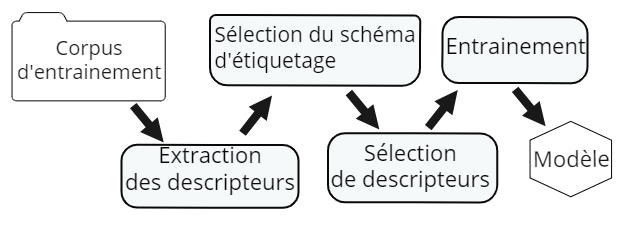
\includegraphics[width=0.8\textwidth]{structuration-training.png}
		\end{figure}
\end{frame}
%\begin{frame}{Définition manuelle des caractéristiques}
%\begin{itemize} \scriptsize
%\item Descripteurs de lignes pour les sections
%\begin{tabular}{|l|l|}
%	\hline
%	\multicolumn{1}{|c|}{Type} & \multicolumn{1}{c|}{Descripteur} \\ \hline
%	Forme &  ses premiers mots  \\
%	& sa longueur absolue  \\ 
%	& sa longueur relative  \\ \hline
%	Contexte & le numéro de ligne  \\
%	&  partie du document contenant la ligne  \\
%	& premiers mots de la ligne précédente  \\ 
%	& ... \\
%\end{tabular}
%\item Descripteur de mots pour les entités
%\begin{tabular}{|l|p{0.78\textwidth}|}
%	\hline
%	\multicolumn{1}{|c|}{Type} & \multicolumn{1}{c|}{Descripteur} \\ \hline
%	Forme &  le mot   \\ 
%	& \og commence-t-il par une lettre majuscule ? \fg{}  \\
%	&\og initiale solitaire ? \fg{}\\
%	& \og S'agit-il d'un mot-clé de règles juridiques ? \fg{}  \\ 
%	& ... \\ \hline
%	Syntaxe & rôle grammatical du mot \\ \hline
%	Sémantique & thème du mot \\ 
%	& ... \\ \hline
%	Contexte & les mots précédents  \\
%	& ... \\ 
%\end{tabular}	
%\end{itemize}
%\end{frame}

\begin{frame}{Résultats}
\begin{figure}
	\begin{itemize}
		\item sélection du schéma d'étiquetage
		\item sélection des descripteurs
	\end{itemize}
\end{figure}
\end{frame}

\subsection{Discussions}
\begin{frame}{Confusions de classes}

\end{frame}


%\begin{frame}{Sélection des caractéristiques}
%\begin{table}[!h]
%\tiny
%\begin{tabular}{l|c|ccc}
%\hline\noalign{\smallskip}
%Detection Task & Tagger & {Token-level F1} & {Entity-level F1}& Features subset \\ \hline
%%\noalign{\smallskip}\svhline\noalign{\smallskip}
%\multirow{7}{*}{Sections} 		& \multirow{4}{*}{CRF} & 99.31 & 90.48 & BDS  \\
%&  & \textbf{99.55} & 85.76 & \textbf{SFFS} \\
%&  & 99.46 & 90.03 & ALL \\
%&  & 91.75 & 60.26 & token \\  \cline{2-5}
%& \multirow{3}{*}{HMM} & \textbf{90.99} & 3.89 & \textbf{absLength} \\ 
%& & 86.97 & 3.65 & relLength \\   
%&  & 37.59 & 18.81 & token \\ \hline
%\multirow{7}{*}{Header entities}	& \multirow{4}{*}{CRF} & 92.69 & 90.47 & BDS  \\
%&  & \textbf{93.00} & 90.76 & \textbf{SFFS}  \\ 
%&  & 92.74 & 90.81 & ALL \\
%&  & 82.73 & 72.17 & token \\ \cline{2-5}
%&  \multirow{3}{*}{HMM}  & \textbf{78.61} & \textbf{56.93} &  \textbf{token} \\ 
%&    & 68.04 & 32.96 &  lemma\_W0 \\ 
%&    & 38.54 & 7.95 &  POS \\ \hline
%\multirow{6}{*}{Norms} 			& \multirow{4}{*}{CRF} & \textbf{96.31} & 90.80 & \textbf{BDS} \\ 
%&  & 95.57 & 89.29 & SFFS \\ 
%&  & 95.87 & 90.76 & ALL \\
%&  & 94.26 & 85.72 & token \\ \cline{2-5}
%&  \multirow{2}{*}{HMM} & \textbf{91.66} & \textbf{74.9} &  \textbf{token} \\ 
%&   & 91.54 & 69.35 &  lemma\_W0 \\ 
%%  \noalign{\smallskip}\svhline\noalign{\smallskip}
%%  & & token-level & entity-level & \\ \hline
%%\noalign{\smallskip}\hline\noalign{\smallskip}
%\end{tabular}
%\caption{Impact de la réduction des caractéristiques}
%\end{table}
%
%%Réduit de \textbf{moitié} le nombre de caractéristiques
%
%%Améliore légèrement les résultats
%
%BDS et SFFS \textcolor{red}{très lents (plus de 10 h lors de nos tests)}
%\end{frame}

\begin{frame}{Nombre nécessaire de données d'entraînement}
\begin{figure}[!h]
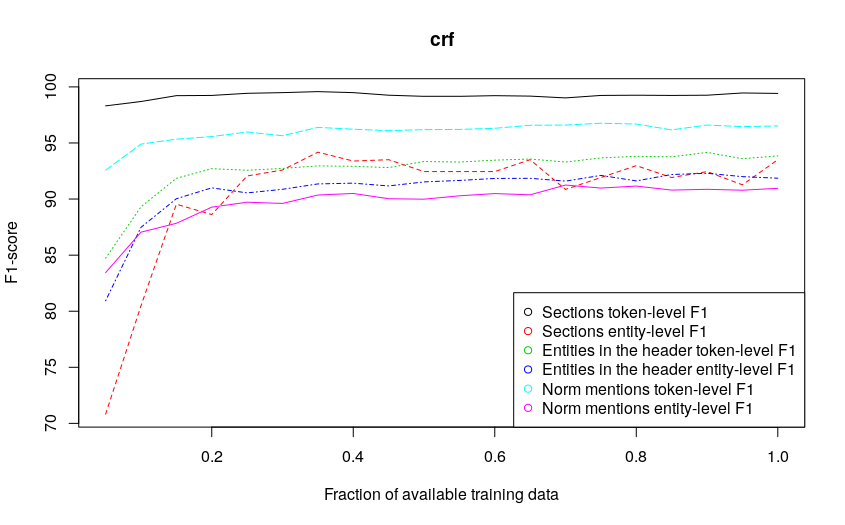
\includegraphics[width=0.9\textwidth]{lc-crf.png}
\caption{Résultats en fonction du nombre de données d'entraînement (fractions d'environ 380 décisions)}\label{p4_crf-learning-curves}
\end{figure}
\end{frame}

\begin{frame}{Description manuelle vs. représentation apprise}

\end{frame}
